\documentclass[11pt]{article}
\usepackage[utf8]{inputenc}
\usepackage{textcomp}
\usepackage{graphicx} 
\usepackage{minted}
\usepackage{xcolor}
\usepackage{amsmath,amssymb}  
\usepackage{bm}
\usepackage[pdftex,bookmarks,colorlinks,breaklinks]{hyperref}  
\usepackage{memhfixc} 
\usepackage{pdfsync}  
\usepackage{fancyhdr}
\usepackage{subcaption}
\pagestyle{fancy}

\newcommand{\norm}[2][2]{\left\lVert #2 \right\rVert_{#1}}

\title{Training the Deep Linear Network}
\author{Dylan Hu}
\date{March 23, 2023}

\begin{document}
\maketitle
{
  \hypersetup{linkcolor=black}
  \tableofcontents
}
\section{Introduction}
With the expansion of computing capabilities driven in large part by innovations in GPUs in the past decade, deep approaches to machine learning formulated decades prior have finally become tractable. Moreover, with the abundance and accessibility of data as well as more complex and powerful model architectures, the impact and potential of deep learning and its applications have gained significant attention (pun intended).
\\\\
In just the past few months, accessible tools powered by deep learning such as ChatGPT have catapulted deep learning into the mainstream. While exciting new developments in deep learning seem to arise each week, we take a step back and analyze some of the fundamental mathematical principles behind deep learning.
\\\\
Arora, Cohen, and Hazan \cite{arora2018optimization} postulate that increased model \textit{depth} not only leads to greater expressiveness, but also that the \textit{overparameterization} leads to implicit acceleration of the optimization.
\\\\
In this report, we investigate and demonstrate the acceleration effect of overparameterization on the optimization of the deep linear network. We also explore further the mathematical basis behind overparameterization through empirical analysis.

\pagebreak

\section{Method}
We build the deep linear network (DLN) as formulated by Arora, Cohen, and Hazan \cite{arora2018optimization}. The DLN is a deep (multi-layer) neural network of $N$ linear layers of size $d \times d$ without activation functions. We therefore may represent the network as a chain of $N$ square $d \times d$ matrices:
$$\bm{W} = \left(W_N, W_{N-1}, \hdots, W_1\right)$$
The observable of the DLN is the product of the matrices in the chain:
$$W := \pi\left(\bm{W}\right) = W_N W_{N-1} \hdots W_1$$
We investigate the acceleration effect of overparameterization by comparing the optimization dynamics of the DLN to that of a single-layer linear network of size $d \times d$, where the chain $\bm{W}$ reduces to the observable $W$ and thus can be considered an end-to-end matrix $W$.

\subsection{Model}
We implement the DLN model in PyTorch:
\begin{minted}[fontsize=\footnotesize]{python}
class DLN(nn.Module):
    def __init__(self, d: int, N: int):
        super().__init__()
        self.d = d
        self.N = N
        self.params = nn.ParameterList(
            [nn.Parameter(torch.randn((d, d))) for _ in range(N)])

    def forward(self) -> Tensor:
        x = torch.eye(self.d)
        for param in self.params:
            x = param @ x
        return x
\end{minted}
\subsection{Optimization}
In investigating the effect of overparameterization on the optimization of the DLN, we consider the optimization problem of matrix completion. Given a random target $d \times d$ matrix $\Phi$, the optimization objective is to find $\bm{W}$ such that the observable $W$ has diagonal entries that match those of $\Phi$.
\\\\
We minimize the following energy functions:
$$E(\bm{W}) = \frac{1}{2} \norm{\text{diag}\left(\Phi - \pi\left(\bm{W}\right)\right)}^2,\quad F(W) = \frac{1}{2} \norm{\text{diag}\left(\Phi - W\right)}^2$$
Note that we distinguish $E\left(\bm{W}\right)$ from $F(W)$, as they have different domains and induce different gradient dynamics for optimization.
\\\\
We denote optimization on the chain of matrices $\bm{W}$ as operating on the ``upstairs'', whereas optimization on the end-to-end matrix $W$ is operating on the ``downstairs''.
\\\\
Training on the upstairs evolves each of the matrices of $\bm{W}$ according to the gradient flow
$$\dot{W}_i = -\nabla_{W_i}E\left(\bm{W}\right)$$
whereas training on the downstairs evolves the end-to-end matrix $W$ by the differential equation
\begin{equation} \label{eq:downstairs}
    \dot{W} = -\frac{1}{N}\sum_{j=1}^N \left(WW^T\right)^{\frac{N - j}{N}} \partial_WF\left(W\right)\left(W^TW\right)^\frac{j - 1}{N}
\end{equation}
where $\partial_WF\left(W\right) = -\text{diag}\left(\Phi - W\right)$.
\subsubsection{Loss function}
We train the DLN upstairs using supervision imposed by a mean-squared-error loss function for which minimization is equivalent to that for the energy function $E\left(\bm{W}\right)$:
$$\mathcal{L_\text{upstairs}} = \text{MSE}\left(\text{diag}\left(\Phi\right), \text{diag}\left(\pi\left(\bm{W}\right)\right)\right) = \frac{1}{d}\sum_{i=1}^d \text{diag}\left(\Phi - \pi\left(\bm{W}\right)\right)_i^2$$
Although this is not the loss function for the downstairs training, we return this loss for both upstairs and downstairs training for the sake of comparison:
$$\mathcal{L_\text{downstairs}} = \text{MSE}\left(\text{diag}\left(\Phi\right), \text{diag}\left(W\right)\right) = \frac{1}{d}\sum_{i=1}^d \text{diag}\left(\Phi - W\right)_i^2$$

\subsubsection{Training upstairs}
The implementation of the upstairs training uses PyTorch's automatic differentiation to compute the gradient of the loss function with respect to the parameters of the DLN. We then update the parameters of the DLN using a built-in optimizer. We experiment with a variety of optimizers, the results of which are discussed in Section \ref{sec:further}.
\begin{minted}[fontsize=\footnotesize]{python}
def upstairs_func(model: DLN,
                  target: Tensor,
                  optimizer: torch.optim.Optimizer,
                  scheduler: Optional[torch.optim.lr_scheduler.LRScheduler]
                    = None):
    def upstairs(train: bool) -> Tensor:
        model.train(train)
        with torch.set_grad_enabled(train):
            optimizer.zero_grad()
            W = model.forward()
            if train:
                loss = F.mse_loss(torch.diag(W), torch.diag(target))
                loss.backward()
                optimizer.step()
                if scheduler:
                    scheduler.step()
                return loss
        return W
    return upstairs

upstairs_model = DLN(d, N) # by default, d = 2, N = 3
optimizer = torch.optim.SGD(upstairs_model.parameters(), lr)
target = torch.randn((d, d))

iteration = 0
upstairs_losses = []

upstairs = upstairs_func(upstairs_model, target, optimizer)
while (loss := upstairs(train=True)) > 1e-7:
    upstairs_losses.append(loss.item())
    iteration += 1
\end{minted}

\subsubsection{Training downstairs}
The downstairs training does not use PyTorch's automatic differentiation but instead uses manual gradient computation and composition according to Eq. \ref {eq:downstairs}.
\begin{minted}[fontsize=\footnotesize]{python}
def downstairs_func(model: DLN, target: Tensor, lr: float, N: int):
    def downstairs() -> Tensor:
        model.train(False)
        with torch.no_grad():
            W = model.forward()
            d_F = torch.diag_embed(torch.diag(W - target))
            WWT = W @ W.T
            WTW = W.T @ W
            d_W = torch.zeros_like(W)
            for i in range(1, N + 1):
                d_W = d_W + \
                    scipy.linalg.fractional_matrix_power(
                        WWT, (N - i) / N) @ \
                    np.array(d_F) @ \
                    scipy.linalg.fractional_matrix_power(
                        WTW, (i - 1) / N)
            d_W = d_W * torch.ones_like(W) / N
            W = W - lr * d_W
            model.params[0] = W
            return F.mse_loss(torch.diag(W), torch.diag(target))
    return downstairs
\end{minted}

\subsection{Further exploration}
\subsubsection{Optimizers}
For the results in Section \ref{sec:results:acceleration}, we use stochastic gradient descent (SGD) for upstairs. However, we also experiment with other optimizers, including Adam and RMSprop. We find that in general, SGD performs best on shallow networks, whereas Adam begins to outperform on deeper networks. The results are shown in Figure \ref{fig:upstairs_optimizers}.

\subsubsection{Learning rate}
We also experiment with different learning rates for both upstairs and downstairs training. As expected, we find that the learning rate has a significant effect on the performance of the DLN, with higher learning rates amenable to shallow networks but not deep networks, where smaller learning rates are required.
\\\\
This reflects the intuition that as the network becomes deeper, the manifold of possible solutions becomes more complex, and the DLN must be more careful in its exploration of the manifold.
\\\\
The results are shown in Figure \ref{fig:lr}.

\subsubsection{Network depth}


\pagebreak

\section{Results}
\subsection{Implicit acceleration} \label{sec:results:acceleration}
\begin{figure}[ht]
    \begin{subfigure}{0.5\textwidth}
        \centering
        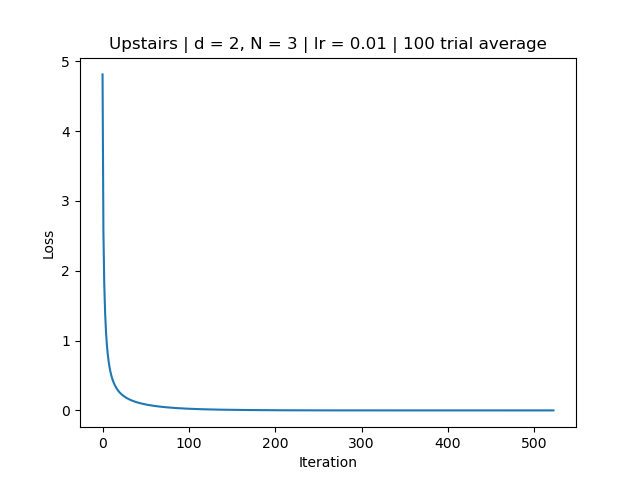
\includegraphics[width=\textwidth]{images/upstairs_avg_lr1e-2.png}
        \caption{100 trial average}
        \label{fig:upstairs_avg}
    \end{subfigure}
    \begin{subfigure}{0.5\textwidth}
        \centering
        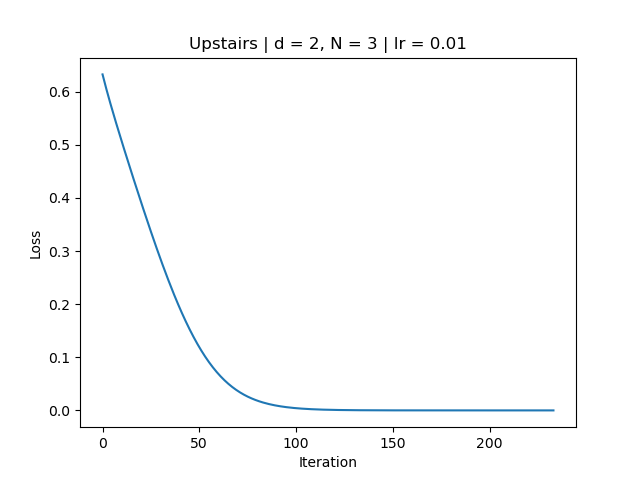
\includegraphics[width=\textwidth]{images/upstairs_1_lr1e-2.png}
        \caption{a particular trajectory}
        \label{fig:upstairs_1}
    \end{subfigure}
    \caption{Training upstairs with $d = 2, N = 3$, and learning rate = 0.01}
    \label{fig:upstairs}
\end{figure}
\begin{figure}[ht]
    \begin{subfigure}{0.5\textwidth}
        \centering
        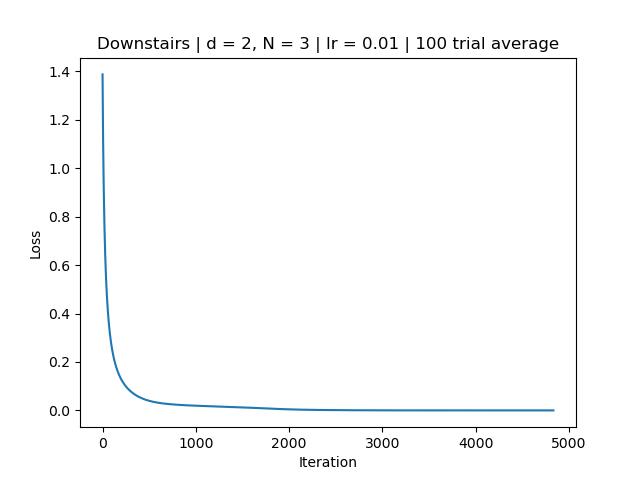
\includegraphics[width=\textwidth]{images/downstairs_avg_lr1e-2.png}
        \caption{100 trial average}
        \label{fig:downstairs_avg}
    \end{subfigure}
    \begin{subfigure}{0.5\textwidth}
        \centering
        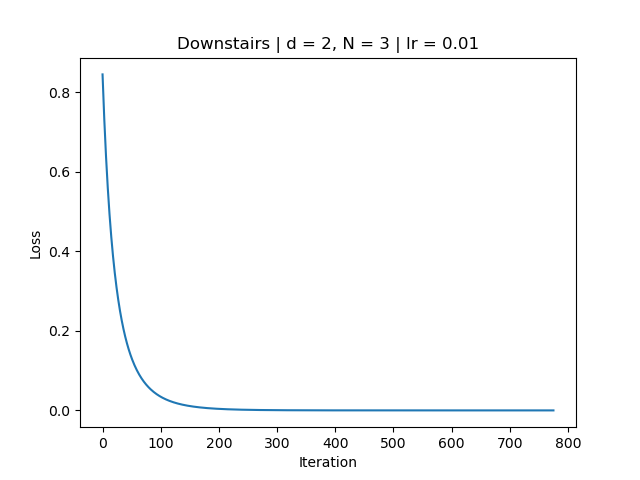
\includegraphics[width=\textwidth]{images/downstairs_1_lr1e-2.png}
        \caption{a particular trajectory}
        \label{fig:downstairs_1}
    \end{subfigure}
    \caption{Training downstairs with $d = 2, N = 3$, and learning rate = 0.01}
    \label{fig:downstairs}
\end{figure}
\subsubsection{Training upstairs}
With $d = 2, N = 3$, and learning rate = 0.01, we are able to successfully train and consistently converge the DLN upstairs using the SGD optimizer. Measured across 100 trials, it takes an average of $204.58$ iterations with standard deviation 101.03 iterations to converge. The average trajectory and a particular trajectory are shown in Figure \ref{fig:upstairs}.

\subsubsection{Training downstairs}
With $d = 2, N = 3$, and learning rate = 0.01, we are also able to successfully train and consistently converge downstairs. However, we find that the convergence is much slower and the trajectory is much more varied than upstairs. Measured across 100 trials, it takes an average of 1410.79 iterations with standard deviation of 1019.89 iterations to converge. The average trajectory and a particular trajectory are shown in Figure \ref{fig:downstairs}.

\subsubsection{Comparison}
We observe that the convergence of the upstairs occurs more quickly and in a more predictable fashion than that of the downstairs, supporting the claim that overparameterization can lead to implicit acceleration. We plot average and particular trajectories for both upstairs and downstairs in Figure \ref{fig:upstairs_downstairs}.
\begin{figure}[ht]
    \begin{subfigure}{0.5\textwidth}
        \centering
        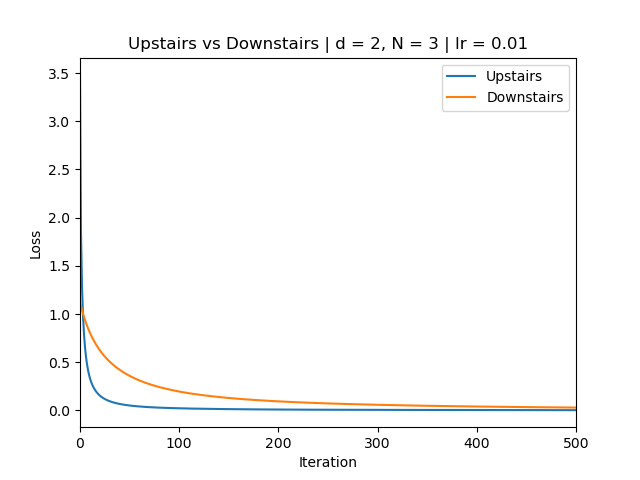
\includegraphics[width=\textwidth]{images/upstairs_downstairs_avg_lr1e-2.png}
        \caption{100 trial average}
        \label{fig:upstairs_downstairs_avg}
    \end{subfigure}
    \begin{subfigure}{0.5\textwidth}
        \centering
        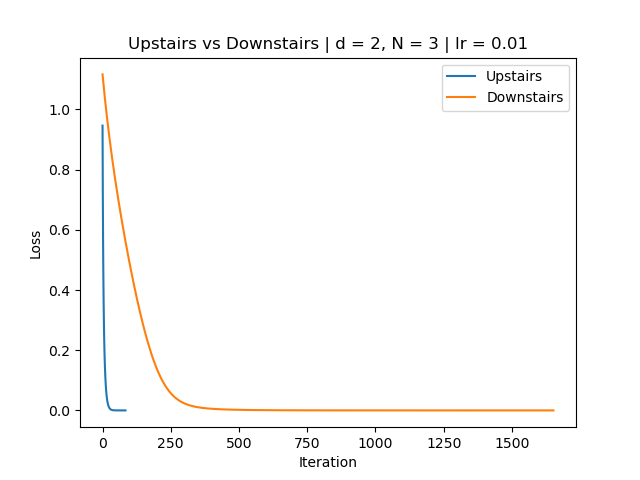
\includegraphics[width=\textwidth]{images/upstairs_downstairs_1_lr1e-2.png}
        \caption{a particular trajectory}
        \label{fig:upstairs_downstairs_1}
    \end{subfigure}
    \caption{Training upstairs compared to downstairs with $d = 2, N = 3$, and learning rate = 0.01}
    \label{fig:upstairs_downstairs}
\end{figure}


\pagebreak

\bibliographystyle{plain}
\bibliography{main}

\end{document}